\section{Allocation of time and resources}
This section presents a complete overview of the available time resources and the distribution of effort that was given to the different subsets of the project. These are further explained in the two next sections.

\subsection{Gantt diagram}
\label{sec:gantt}

A Gantt diagram gives an overview of the overall timeline of a project. The diagram orders items chronologically to easily show the predicted state of the project. These items can represent milestones, sprints, deadlines and team downtime. 

The Gantt diagram for the project is shown in figure~\ref{fig:gantt}. The sprints are shown as blue rectangles. The red rectangle indicates the school trip to China in April that the whole team attended. The blue diamonds indicate milestones, or deadlines for delivery of some major part of the project.


\begin{figure}[H]
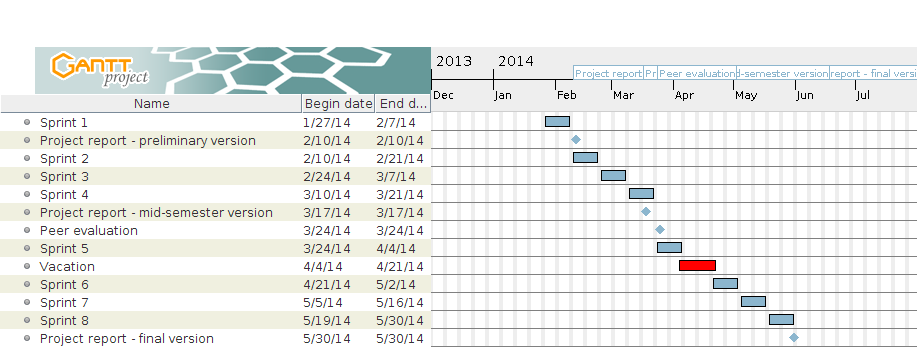
\includegraphics[width=\textwidth]{ch/projectManagement/fig/gantt.png}
\caption{The Gantt diagram with sprints and milestones}
\label{fig:gantt}
\end{figure}


\subsection{Work Breakdown Structure}
\label{sec:wbs}

\begin{figure}[H]
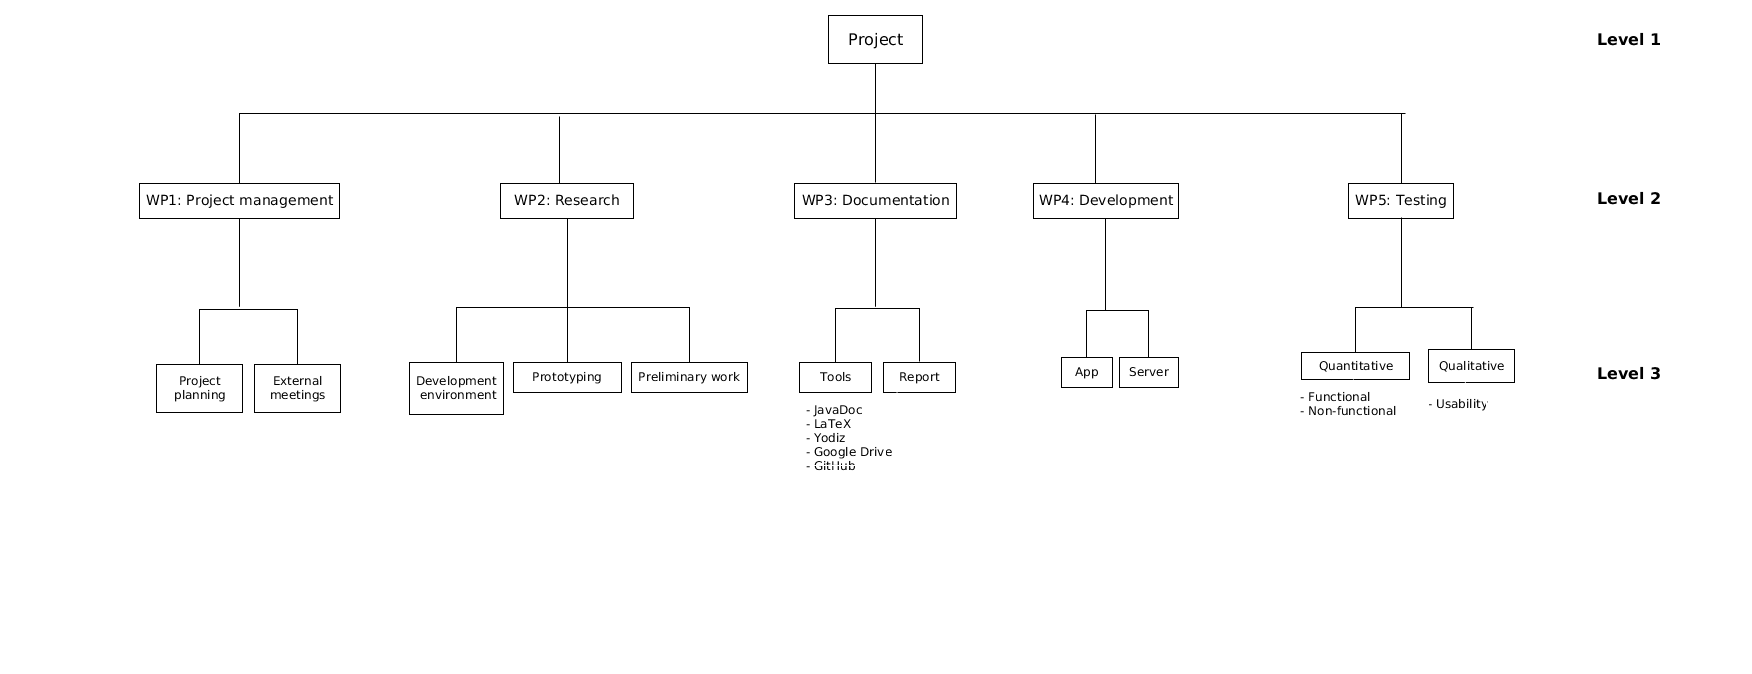
\includegraphics[width=\textwidth, trim=9.5cm 6cm 8.5cm 0.9cm,clip]{ch/projectManagement/fig/wbs2.png}
\caption{Product oriented work breakdown structure for the project app}
\label{fig:wbs}
\end{figure}

As shown in figure~\ref{fig:wbs}, the Work Breakdown Structure (WBS) is divided into five work packages. Each work package represents a subset of the project. Specifically, it specifies \emph{what} will be done, and not how or when the work is to be performed.

The team used WBS in order to get an overview of what kind of work the different parts of the project consisted of, and used this information to estimate how much time to use on each work package.

The estimated time for each work package is given in table~\ref{tab:timeEstWP}. By comparing the time estimates to the actual time spent, it was possible to evaluate the project's progress to a much greater extent. It was easier to see whether some part of the project was neglected. This comparison is done in section~\ref{sec:timeSpent}.


\begin{table}[H]
\centering
\rowcolors{1}{darkgray}{lightgray}
\begin{tabular}{|l|l|c|l|}
\hline
    \textbf{Work Package \#} & \textbf{Name} & \textbf{\%} & \textbf{Hours} \\\hline
    1 & Project management & 5 & 87\\\hline
    2 & Research		   & 15 & 261\\\hline
    3 & Documentation	   & 40 & 696\\\hline
    4 & Development 	   & 30 & 522\\\hline
    5 & Testing  		   & 10 & 174\\\hline
\end{tabular}
\caption{Time estimate for work packages}
\label{tab:timeEstWP}
\end{table}
